\subsection{Network Layer Routing Algorithms}

A graph \(\function{G}{N, E}\) comprises a set of routers \(N\) and a set of links \(E\) between those routers.
The cost of a link between routers~\(x\) and \(y\) is expressed as \(\function{c}{x, y}\).
The cost of a link could always be \num{1}, or could be inversely related to bandwidth or congestion.
A routing algorithm finds the least-cost path between two routers.

\subsection{Classification of Routing Algorithms}

A routing algorithm in which topology and link cost information is shared globally between all routers is known as a `link-state' algorithm.
A decentralised routing algorithm in which a router knows only the link costs to its neighbours and communicates information only with its neighbours is known as a `distance-vector' algorithm.

A routing algorithm in which routes change slowly over time is a static algorithm, whereas an algorithm in which routes change quickly with periodic updates and responses to link cost changes is a dynamic algorithm.

\subsection{Link-State Routing (Dijkstra's Algorithm)}

Dijkstra's algorithm is a link-state routing algorithm in which the network topology and link costs are known to all nodes.
This is accomplished via link-state broadcast.
All nodes have the same information.
The least-cost paths from the source node to all other nodes is computed to provide a forwarding table for that node.
The algorithm is iterative; after \(k\) iterations, the least-cost paths to \(k\) destinations are known.

\begin{itemize}
  \item \(\function{c}{x, y}\) --- link cost from node~\(x\) to node~\(y\), infinite cost if not direct neighbours
  \item \(\function{D}{v}\) --- current cost of path from source to node~\(v\)
  \item \(\function{p}{v}\) --- predecessor of node~\(v\) along path from source to node~\(v\)
  \item \(N'\) --- set of nodes whose least-cost paths are definitively known
\end{itemize}

\begin{enumerate}
  \item Add source node~\(u\) to \(N'\)
  \item For all nodes~\(v\), if \(v\) is adjacent to \(u\), set \(\function{D}{v} = \function{c}{u, v}\), else set \(\function{D}{v} = \infty\)
  \item Find the node~\(w\) not in \(N'\) with the least \(\function{D}{w}\)
  \item Add node~\(w\) to \(N'\)
  \item Update \(\function{D}{v}\) for all nodes~\(v\) adjacent to \(w\) and not in \(N'\) such that \(\function{D}{v} = \function{min}{\function{D}{v}, \function{D}{w} + \function{c}{w, v}}\)
  \item Repeat from step~\num{3} until all nodes are in \(N'\)
\end{enumerate}

\begin{figure}[htp]
  \centering
  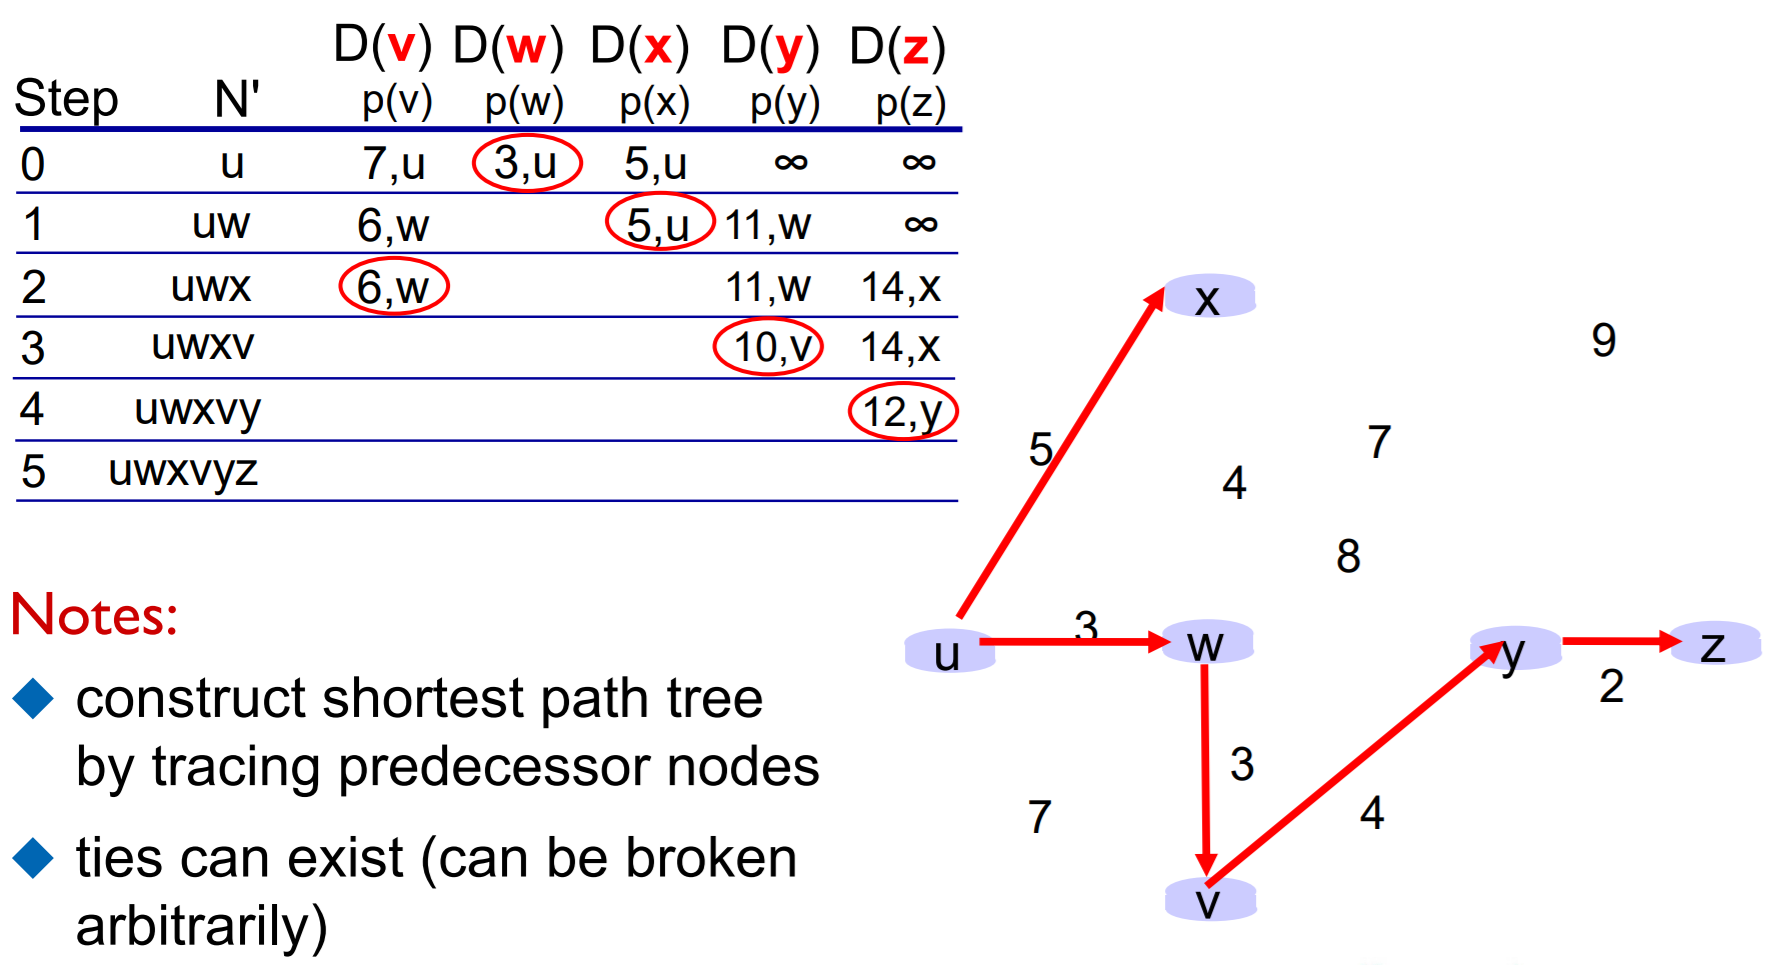
\includegraphics[width=15cm]{unit-19/figures/dijkstras-algorithm.png}
  \caption*{Example of Dijkstra's algorithm.}
\end{figure}

Each iteration requires all nodes not in \(N'\) to be checked.
This is \(n \left(n + 1\right)\) comparisons.
Thus, the algorithm has complexity class \(\function{O}{n^2}\), although more efficient implementations are possible.

In a network in which link cost is determined by traffic, Dijkstra's algorithm can result in oscillations.
If all routers simultaneously direct all traffic along the least-cost paths, those paths will become the greatest-cost paths.
The routers would then direct traffic along the next least-cost paths, continuing the cycle.

To solve this problem, routers could employ the algorithm at different times rather than simultaneously.
However, routers will tend to synchronise over time.
A better solution is not to base link cost solely on network traffic.

\subsection{Distance-Vector Routing (Bellman-Ford Algorithm)}

Distance-vector routing can be employed using the Bellman-Ford equation.
The cost of the least-cost path from node~\(x\) to node~\(y\) is the minimum, taken over all neighbours \(v\) of \(x\), of the sum of the cost to neighbour~\(v\) and the cost from neighbour~\(v\) to destination~\(y\).

\begin{equation*}
  \functionsub{d}{x}{y} = \functionsub{min}{v}{\function{c}{x, v} + \functionsub{d}{v}{y}}
\end{equation*}

The node achieving the minimum is the next hop in the shortest path used in the forwarding table.

The function \(\functionsub{D}{x}{y}\) is an estimate of the least cost from \(x\) to \(y\).
Node~\(x\) knows the cost to each neighbour~\(v\) and maintains its distance vector \(\mathbf{D}_x = \functionsub{D}{x}{y}\) for all \(y\) in \(N\).
It maintains a copy of the distance vectors of its neighbours.
For each neighbour~\(v\), \(x\) maintains a distance vector \(\mathbf{D}_v = \functionsub{D}{v}{y}\).

Periodically, each node sends its own distance vector estimate to its neighbours.
When a node~\(x\) receives a new estimate from its neighbour, it updates its own distance vector using the Bellman-Ford equation.
Under natural conditions, the estimate \(\functionsub{D}{x}{y}\) converges to the actual least cost \(\functionsub{d}{x}{y}\).

The distance-vector algorithm is iterative and asynchronous.
Each local iteration is caused by a local link cost change or a distance-vector update message from its neighbour.
The node updates its routing info and recalculates its distance vector.
It notifies its neighbours only when its distance-vector changes.

One drawback of the distance-vector algorithm is that an increase in link cost does not trigger notification message.
The network continues to operate as if cost had not increased.

\begin{figure}[htp]
  \centering
  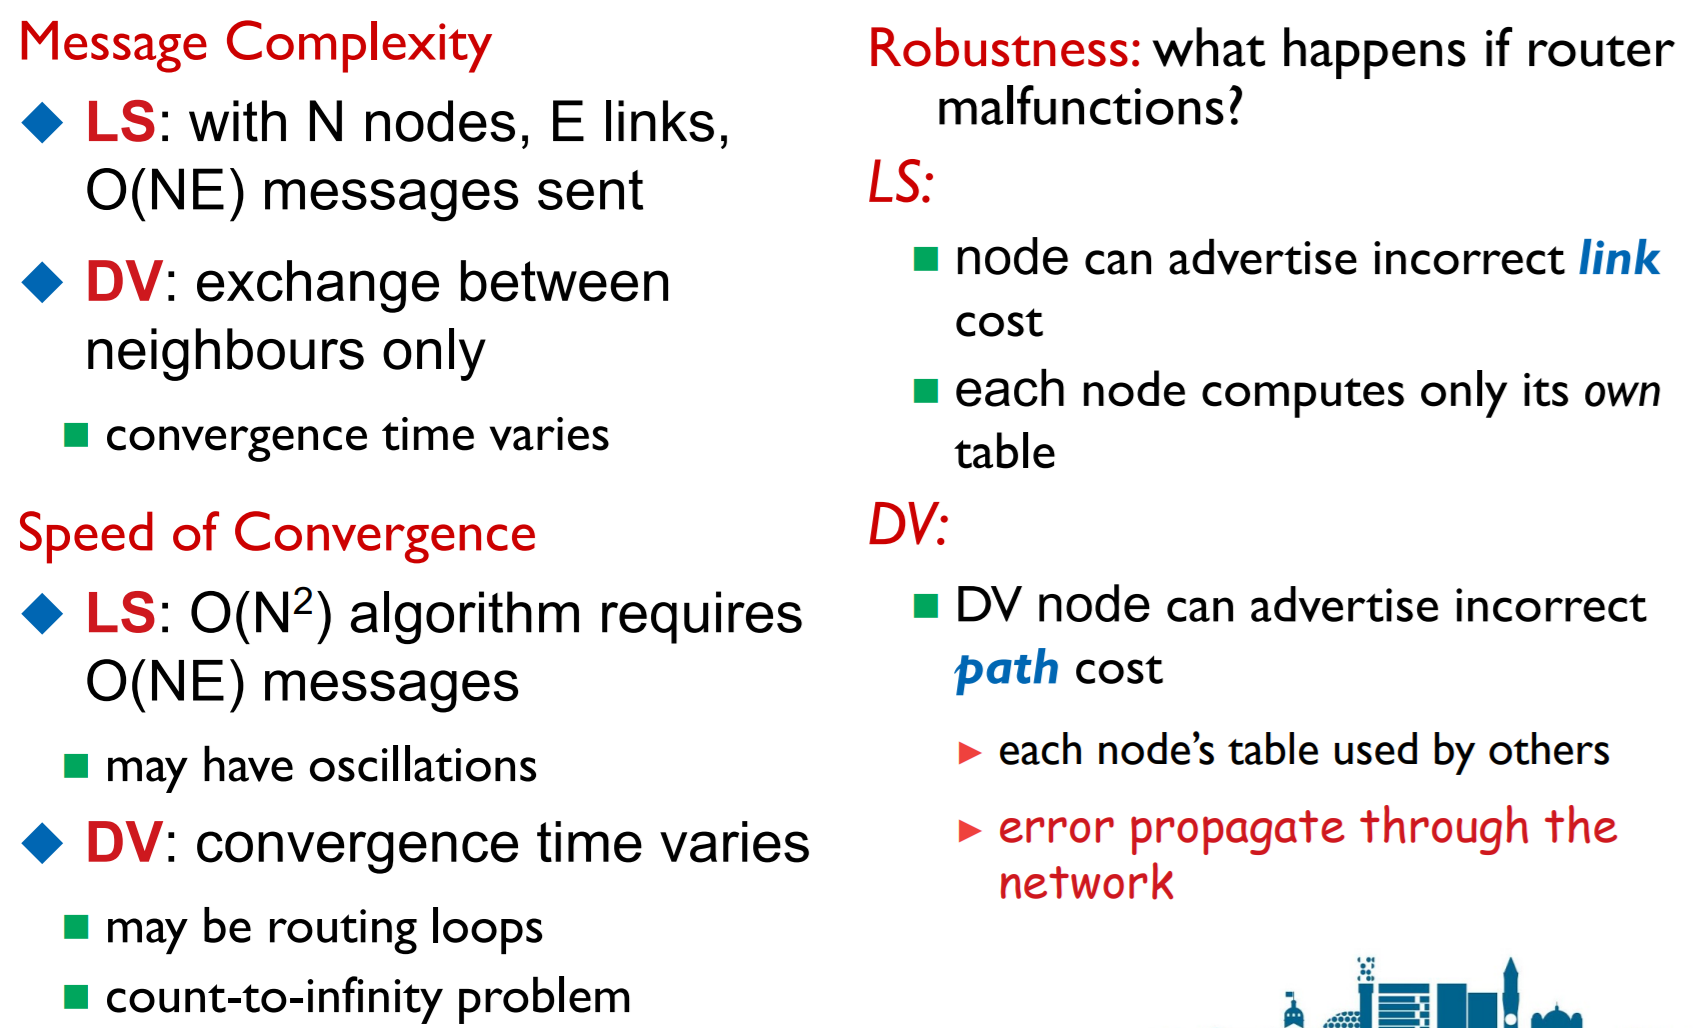
\includegraphics[width=12cm]{unit-19/figures/routing-algorithms.png}
  \caption*{Comparison of link-state and distance-vector algorithms.}
\end{figure}

\subsection{Hierarchical Routing}

In reality, not all routers are identical and there are millions of destination address that cannot all be stored in routing tables.
The exchange of so many routing tables would significantly harm the performance of the Internet.
Additionally, the administrators of each network in the Internet may want to control routing within their own network.

Routers are aggregated into regions known as autonomous systems (AS).
Routers within the same AS run the same routing protocol.
This is known as the `intra-AS' routing protocol.
Routers in different autonomous systems can run different intra-AS routing protocols.
A gateway router is a router at the edge of its AS that has a link to another AS\@.

The forwarding table of a router is configured by both intra-AS and inter-AS routing protocols.
Entries for internal destinations are set by the intra-AS protocol.
Entries for external destinations are set by both the intra-AS and inter-AS protocols.

It is the job of the inter-AS protocol to learn which destinations are reachable through each gateway router, and to propagate this information within its AS\@.
If an external destination is reachable through more than one gateway, the inter-AS protocol may use ``hot-potato routing'' to send the packet to the closest gateway.

\begin{figure}
  \centering
  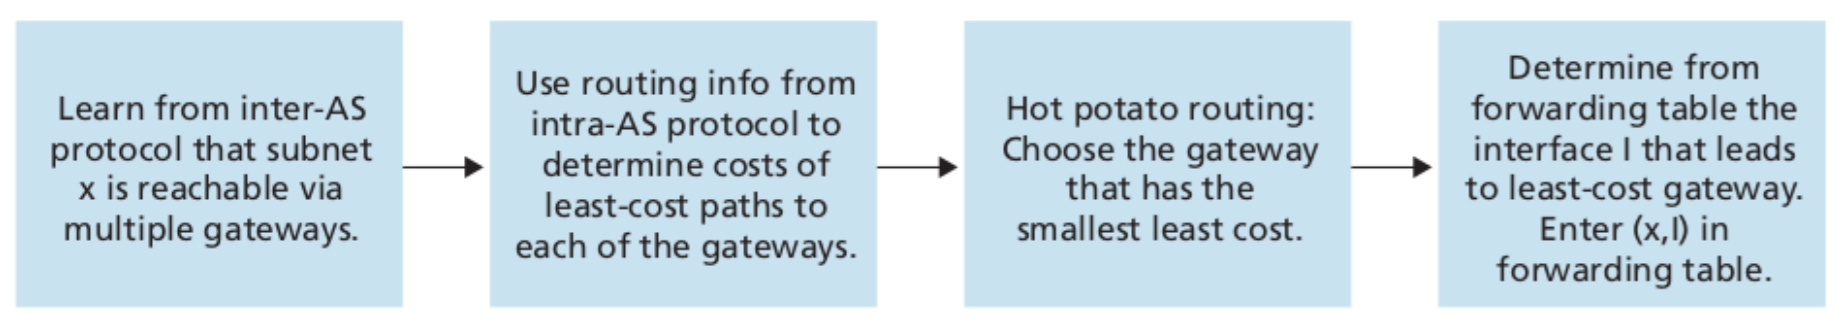
\includegraphics[width=15cm]{unit-19/figures/hot-potato.png}
  \caption*{Multiple gateways and hot-potato routing.}
\end{figure}
